\documentclass[10pt]{article}
\usepackage{verbatim}
\usepackage{multirow}
\usepackage{fullpage}
\usepackage{graphicx} 
\usepackage{float}
\usepackage{url}

\bibliographystyle{IEEEtran}

\pagestyle{plain}

\title{{\normalsize CSCI 572:  Computer Networks II (Fall 2023)}\\Smart Bandwidth Allocation: 
Using ML for Home Networks
}
\author{Yichong Liang, Ping Zhang}

\begin{document}
\maketitle

\section{Introduction}
% Motivate the problem;
% Define/formulate the problem: assumptions, application requirements, goals and non-goals;
\subsection{Overview}
\paragraph{}
As home networks grow more complex with an increasing number of devices requiring bandwidth simultaneously, there arises a pressing need to manage and optimize bandwidth allocation efficiently. This project aims to harness the power of machine learning to predict bandwidth requirements and dynamically allocate resources based on the behavior patterns and usage trends of family. Let's consider a scenario where a family of four, consisting of two adults and two children of varying ages, resides in a home. How these Four individuals use their internet devices throughout the 5:00 pm - 11: 00pm. Based on these usage patterns, we dynamically allocate resources to the regularly used devices during specific time periods to enhance network resource utilization and improve user experience.
\subsection{Motivation}
\paragraph{}
The motivation often arises from a combination of ``people problems'' (real-world issues affecting individuals or society) and ``technical problems'' (limitations or challenges associated with current technologies or methodologies). 

\paragraph{}
\textbf{People Problems:} The ``people problems'' typically relates to how the issue at hand affects users or stakeholders. For instance, in the context of smart bandwidth allocation using machine learning: Users may experience slow internet speeds due to inefficient bandwidth allocation. There might be a lack of fairness in bandwidth distribution among family members, leading to frustration or conflict. As more devices connect to home networks, users may find it increasingly difficult to manage their network settings manually. These problems are not trivial because: User behavior is diverse and unpredictable, making static bandwidth allocation ineffective. Manual adjustments to network settings are time-consuming and impractical for non-technical users. The number of devices and the demand for bandwidth are continuously increasing, exacerbating the problem.

\paragraph{}
\textbf{Technical Problems:} The technical problem often involves the limitations of current solutions in addressing the people problem effectively. For the smart bandwidth allocation, existing routers and network management systems may not be sophisticated enough to dynamically allocate bandwidth based on real-time needs and predicted usage patterns.Traditional network setups may not incorporate machine learning algorithms that can learn and adapt to user behavior over time. Previous solutions may not scale well with the increasing number of devices and the complexity of network traffic.
These technical issues prevent a trivial solution because Simple rules-based systems cannot capture the complexity and dynamic nature of modern home networks. Upgrading network infrastructure to support better bandwidth management can be prohibitively expensive or technically challenging. There is a need for intelligent systems that can operate autonomously, require minimal user intervention, and can adapt to changing network conditions.


\subsection{Assumptions}
\begin{itemize}
  \item \textbf{User Behavior Consistency}: Family members’ behavior in content consumption is somewhat consistent over time in certain scenario, allowing for predictive patterns to be discerned.
  \item \textbf{Data Quality}: The data collected from devices is accurate, timely, and free from corruption or tampering.
  \item \textbf{Network Stability}: The home network is stable and reliable, with minimal unexpected downtimes or disruptions.
  \item \textbf{Device Homogeneity}: All devices in the network can communicate seamlessly with the local server or middleware without compatibility issues.
  \item \textbf{Privacy and Security}: Family members are aware of and consent to the data collection. The system’s internal security measures are sufficient to prevent unauthorized access.
  \item \textbf{ML Model Assumptions}: Features chosen for the ML model are relevant and have a direct impact on predicting network usage.
  \item \textbf{Network Limitations}: There is a consistent and predictable upper limit to the home network’s bandwidth.
\end{itemize}

\subsection{Project Objectives and Constraints}
\paragraph{Goals}
\paragraph{}
The primary goals of a network management system designed to analyze, predict, optimize, and adapt to the evolving bandwidth needs of a family.

\begin{itemize}
  \item \textbf{Analyzes}: Captures real-time data on device activities, time of usage, and specific bandwidth-heavy tasks, correlating them with specific family members’ habits.
  \item \textbf{Predicts}: Utilizes machine learning algorithms to anticipate when high bandwidth periods are likely based on family behavior, thus enabling pre-emptive allocation.
  \item \textbf{Optimizes}: Allocates bandwidth based on predicted needs, ensuring high-priority tasks have necessary bandwidth, reducing lag and ensuring efficient network performance.
  \item \textbf{Adapts}: As family behavior evolves, the system learns from new data and feedback. It refines its predictions and bandwidth allocation strategies to better serve the evolving needs of the family, preventing bottlenecks before they can happen.
\end{itemize}

\paragraph{Non-Goals}
\begin{itemize}
    \item \textbf{Machine Learning Integration:} The project does not aim to integrate complex Machine learning models, focusing instead on use existing, proven machine learning techniques rather than developing entirely new algorithms suitable for home networks.
    
    \item \textbf{Specific Content Prediction:} The primary objective is bandwidth allocation, not predicting the specific content that users might access.
    
    \item \textbf{Infrastructure Overhaul:} The project does not intend to replace or drastically modify existing home network infrastructure but rather aims to enhance its performance.
    
    \item \textbf{Addressing Wide Area Networks:} The project is centered on home networks, so challenges specific to wide area networks or large-scale infrastructures are not addressed.
\end{itemize}


\section{Related work}
   %\item What has been done before?
%\item How does your solution compare to them?
\paragraph{}   
After browsing through some resources and filtered article that publish after 2019. Have
noticed that there are some research had conducted under similar concept. Hatem’s\cite{hatem2019}, Wang’s\cite{wang2020}, and this proposal, focus on optimization. Hatem’s article emphasizes optimizing bandwidth in NG-EPONs, Wang’s is about optimizing video stream analytic at the edge, and this solution revolves around optimizing bandwidth allocation in home networks. All of these try to use the leverage of machine learning to predict and optimize.

\paragraph{}
The three concepts aim to reduce unnecessary overhead and latency in their respective domains. Hatem seeks to decrease the control overhead in NG-EPONs, Wang’s approach tries to cut down on latency by employing edge computing, and this solution targets seamless
content delivery in home networks.

\paragraph{}
For the differences of each concept and solution, the solution I proposed is particularly tailored for home network environments. Unlike the intensive deep learning approach of Hatem or the algorithmic complexity presented by Wang, the proposal approach is cognizant of the fact that home networks may not have the computational resources comparable to dedicated optical networks or edge servers. Thus, this solution is designed to be less computationally intensive, ensuring it’s feasible and effective for residential settings.

\paragraph{}
Which aim to do this without imposing heavy computational burdens that could potentially slow down the network or require additional, often expensive, hardware upgrades.The approach is intended to be integrated directly into existing home network systems. By harnessing machine learning in a manner that isn’t overly resource intensive, the proposal solution offers an efficient, practical way to improve bandwidth allocation in everyday residential networks.

\section{Approach} %(optional)

\paragraph{}
The rationale behind the project hinges on the ever-growing reliance on home networks, which are increasingly burdened by high-bandwidth activities like video streaming, online gaming, and telecommuting. This project addresses the common issue of inconsistent network performance by developing a system that intelligently allocates bandwidth. By understanding and predicting usage patterns, the network can dynamically adjust to provide a seamless online experience for all users.

\paragraph{}
The approach begins with an in-depth analysis of the family’s digital lifestyle, encompassing their online activities ranging from streaming high-definition videos to casual web surfing. This initial phase is critical to gain a comprehensive understanding of the typical network demands within the household.

\paragraph{}
Simultaneously, a thorough evaluation of the family's network setup is conducted. This involves cataloging all connected devices, from smartphones to smart home appliances, and assessing their individual and collective bandwidth consumption. This step is crucial for building a complete picture of the network's load at any given time.

\paragraph{}
The next phase focuses on implementing sophisticated logging tools across these devices. These tools are designed to meticulously monitor network usage patterns and bandwidth consumption in real-time. This phase is pivotal in collecting the raw data needed for later analysis.

\paragraph{}
A detailed observation strategy is adopted, where the network's bandwidth consumption is tracked meticulously across various devices. This monitoring occurs at different times of the day to capture a diverse range of usage scenarios. The aim here is to pinpoint peak usage periods, identify high-bandwidth devices, and determine which applications or services are the most demanding in terms of network resources.

\paragraph{}
Upon gathering a substantial amount of data, the next step involves a rigorous process of data cleaning, standardization, and anomaly detection. This process ensures that the data fed into the subsequent stages is accurate and reliable.

\paragraph{}
With a refined dataset at hand, the project moves into the realm of machine learning. Here, various models are developed and trained to accurately predict future bandwidth requirements based on observed user behavior patterns. The ideal model would be capable of forecasting network demands in real-time, facilitating dynamic bandwidth allocation.

\paragraph{}
The project then leverages the capabilities of the NS-3 simulator to test a range of bandwidth allocation strategies informed by the machine learning model. This simulated environment is crucial for understanding the potential impacts of different allocation strategies on network performance, particularly in scenarios where multiple devices are accessing the network simultaneously.


\subsection{Roadmap}
\paragraph{}
The roadmap of the approach as Figure 1 - Approach Roadmap.
\begin{figure}[H]
    \centering
    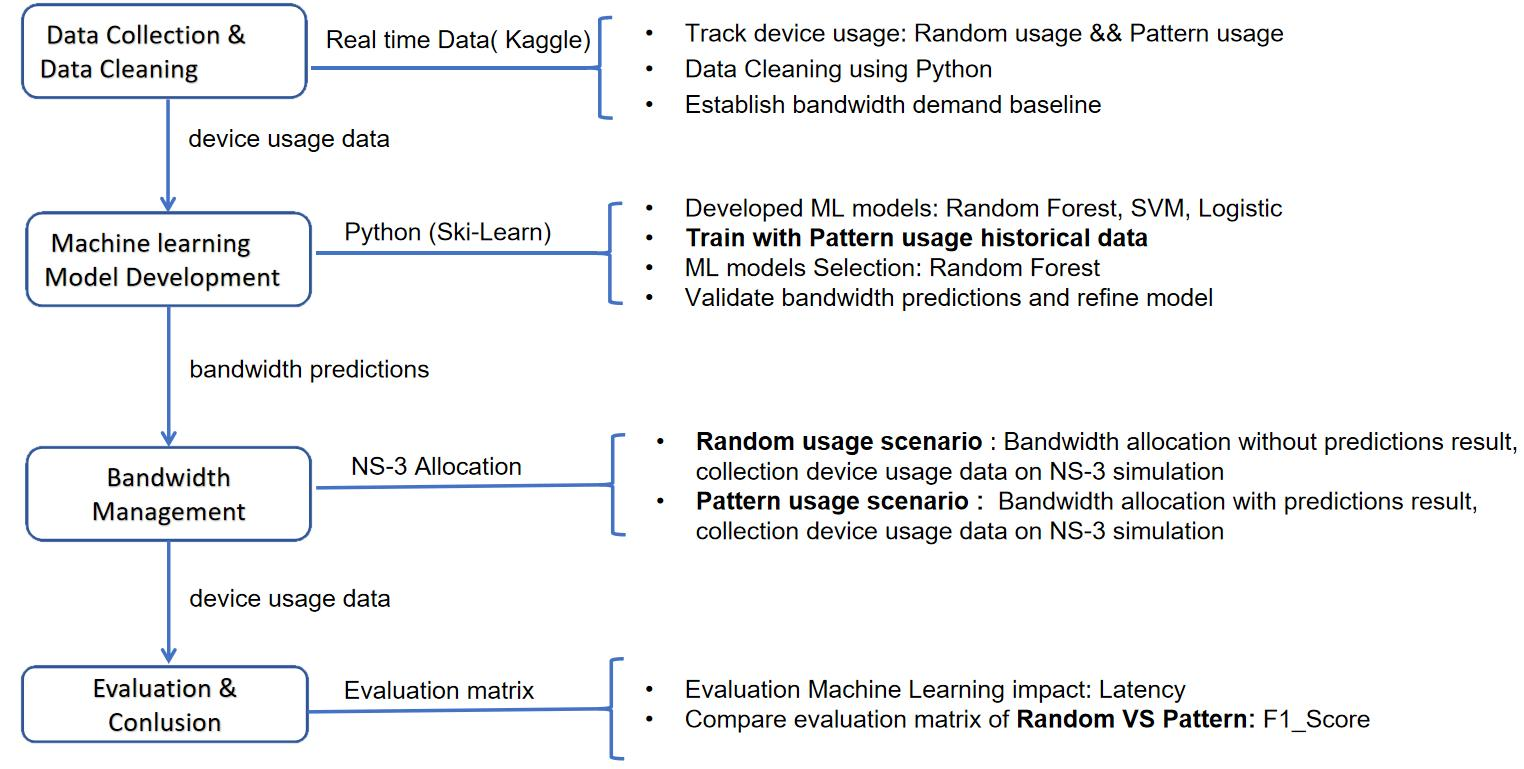
\includegraphics[width=1\linewidth]{Approach Roadmap.jpg}
    \caption{Approach Roadmap}
    \label{fig:enter-label}
\end{figure}
\begin{enumerate}
  \item \textbf{Step 1 - Data Collection}: Implement real-time network traffic analysis to capture live bandwidth usage. This involves tracking the activity of each device on the network to discern patterns of high and low usage. Utilized data sets available on platforms like Kaggle \cite{navabhaarathi2023network} to supplement real-time data, ensuring a robust data set for model training. After that apply data preprocessing techniques using Python to clean and organize the data set. This step is crucial to remove outliers, handle missing values, and ensure the data set's quality.
  \item \textbf{Step 2 - Machine Learning Model}:  Experiment with various machine learning algorithms such as Random Forest, Support Vector Machine (SVM), and Logistic Regression to determine the most effective model for predicting bandwidth usage. Then Leverage historical data of pattern usage to train the ML models, ensuring they can accurately predict future demands based on past behavior. After that continuously validate and refine the model's predictions by comparing them against actual usage patterns to improve accuracy over time.
  \item \textbf{Step 3 - Bandwidth Management}: Use the NS-3 network simulator to apply the ML model's predictions for bandwidth allocation in various scenarios, including random usage and pattern usage. Contrast the effectiveness of bandwidth allocation with and without the ML predictions to assess the impact of ML-informed decisions.
  \item \textbf{Step 4 - Evaluation}: 
  \begin{enumerate}
    \item Compare the network latency in scenarios of random usage versus pattern-based usage to determine if ML predictions result in lower latency. Utilize the F1\_Score, which combines precision and recall, to gauge the accuracy of the ML model. An F1\_Score close to 1 indicates a highly accurate model.
    \item Use data results from NS-3 simulations to inversely validate the Machine Learning Model, resulting in an F1\_Score to assess the model's accuracy. The expected result is that the latency of pattern usage is less than the latency of random usage, and the F1\_score of the ML model is close to 1.
  \end{enumerate}
\end{enumerate}



\section{Implementation}

\subsection{Contrast Experimental scenario}
\paragraph{}
The project Design Contrast Experimental scenario :  Random Scenario  VS  Pattern Scenario. These contrasting setups are crucial for assessing the benefits of using a machine learning model for dynamic bandwidth management in home networks.

\paragraph{}
\textbf{Random Scenario  (Figure 2):} 
In the random scenario, the network is challenged by the unpredictable use of devices between 5:00 PM and 11:00 PM, with no set patterns, leading to potential bandwidth contention and performance issues. 

\paragraph{}
\textbf{Pattern Scenario (Figure 3):}
The pattern scenario depicts a structured device usage within the same hours, allowing for more predictable and efficient bandwidth allocation, likely resulting in improved network performance and lower latency.  

\begin{figure}[H]
    \centering
    \begin{minipage}{0.48\linewidth}
        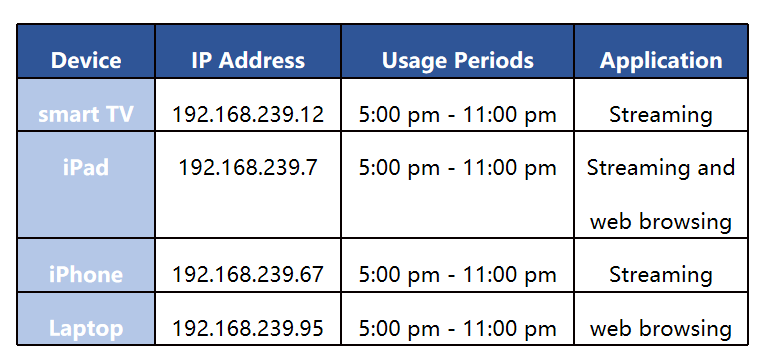
\includegraphics[width=\linewidth]{Random Scenario design.png}
        \caption{Random Scenario design}
        \label{fig:random-scenario}
    \end{minipage}\hfill
    \begin{minipage}{0.48\linewidth}
        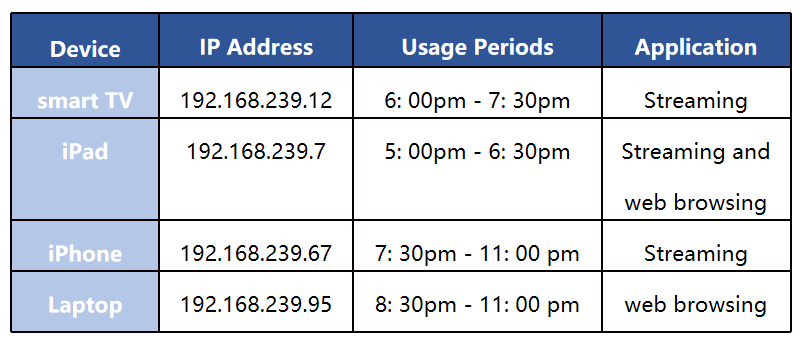
\includegraphics[width=\linewidth]{Pattern Scenario design.png}
        \caption{Pattern Scenario design}
        \label{fig:pattern-scenario}
    \end{minipage}
\end{figure}


\subsection{Machine Learning Model Building}
\paragraph{}
The flowchart (Figure 4) illustrates process of model training. Which involves data collection and cleaning, splitting the data into inputs and targets, building a model, training the model with training data using various machine learning algorithms, testing the model with test data, and evaluating the model's performance using the F1 score metric.
\begin{figure}[H]
    \centering
    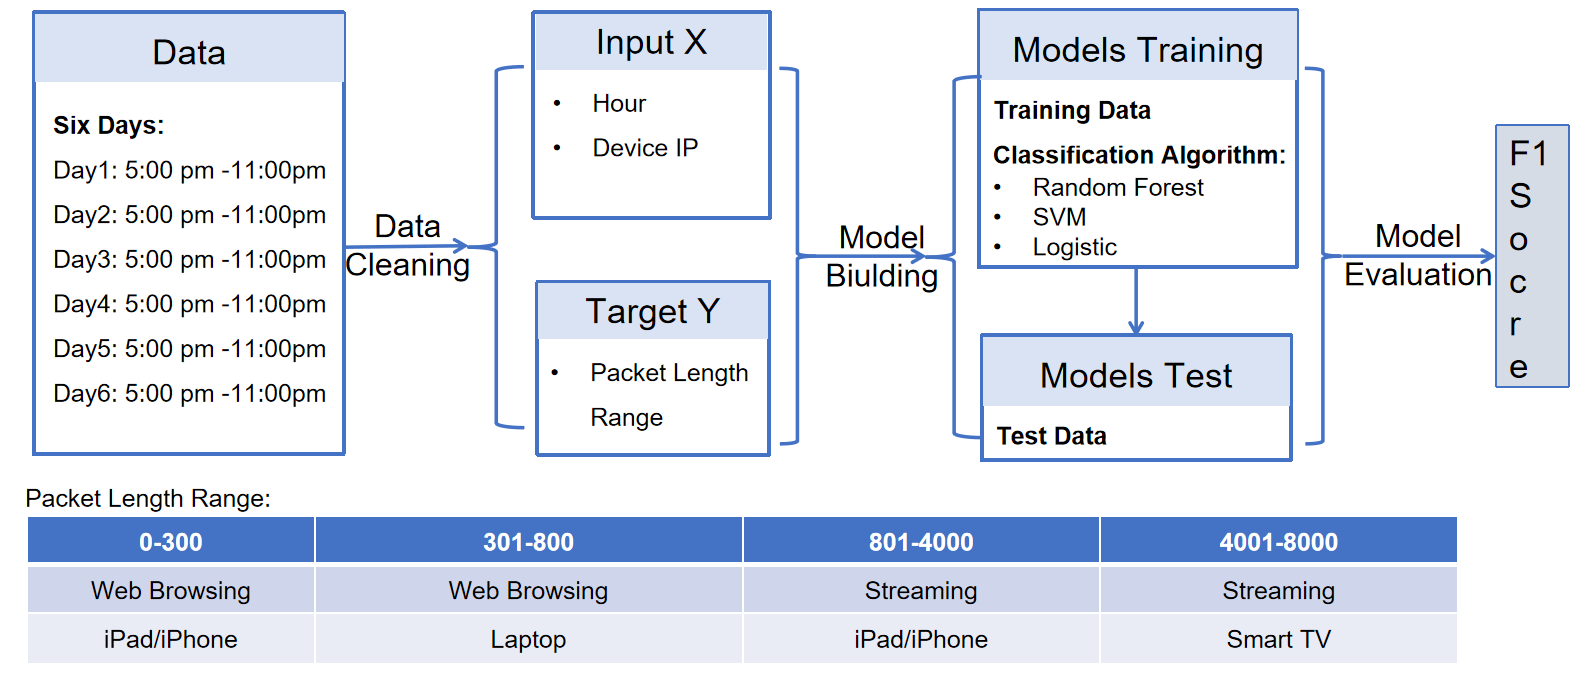
\includegraphics[width=0.9\linewidth]{Machine Learning Model Building.png}
    \caption{Machine Learning Model Building}
    \label{fig:enter-label}
\end{figure}
\paragraph{}
Over a period of six consecutive days, network traffic data is collected from 5:00 PM to 11:00 PM, capturing the peak usage hours for most households. This data includes the packet lengths transmitted by various devices connected to the home network. 0-300 for ipad iphone for some basic web browsing,  laptop 300-800 for maybe heavier browsing tha might contain images, 800-4000 for streaming on ipad iphone which is quite enough for some youtube or short video 4000-8000 for TV for heavy streaming. The raw data is then subjected to cleaning processes to ensure its quality. This involves filtering out irrelevant information, correcting errors, and handling missing values, which prepares the data for effective analysis and modeling.

\paragraph{}
The cleaned data is split into two parts: Input X and Target Y. Input X consists of features like the hour of the day when the traffic was recorded and the IP addresses of the devices, which act as predictors. Target Y is the outcome variable and includes the range of packet lengths, categorized by the type of activity and the device being used.

\paragraph{}
With the data prepared, the next step is to build the classification machine learning model. This involves selecting the appropriate algorithms that will be used to predict the packet length range based on the input features. The chosen algorithms for this process include Random Forest, Support Vector Machine (SVM), and Logistic Regression. The selected models are trained using the training data, which is a subset of the cleaned data. During training, the models learn to associate the input features with the target variable by finding patterns in the data.

\paragraph{}
After training, the models are tested using a separate subset of the data known as test data. This step is critical for assessing how well the model can generalize to new, unseen data. Finally, the model's performance is evaluated using the F1 Score.

\newpage
\subsection{Machine Learning Model Selection}
\paragraph{}
From the random behavior scenario, it is observed that neither Random Forest nor Logistic Regression models achieve ideal performance across all categories. The SVM model is too computationally intensive so it's been remove from comparison.

\paragraph{}
In the pattern behavior scenario, all three models Random Forest, SVM, and Logistic Regression demonstrate significantly better outcomes. Notably, the Random Forest model stands out with superior performance across all categories, which suggests its robustness in handling structured and predictable patterns in the dataset.

\paragraph{}
The disparity in model performance between random and pattern scenarios is expected. In random scenarios, unpredictability in data can make it challenging for models to learn and make accurate predictions. Conversely, pattern scenarios with structured and consistent data allow models to detect underlying patterns and improve their predictive performance.

\paragraph{}
The choice to proceed with Random Forest for further development is based on its comprehensive coverage across all categories and its robust performance in the face of varied data patterns. 

\begin{figure}[H]
    \centering
    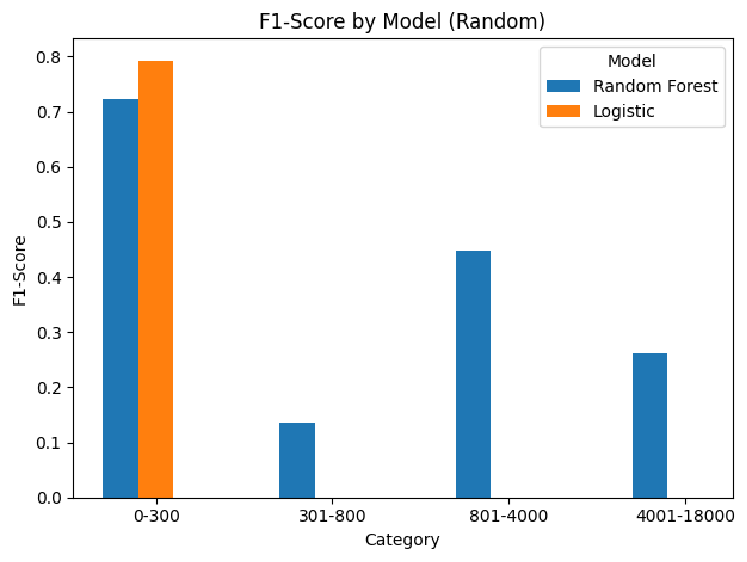
\includegraphics[width=0.7\linewidth]{Random Scenario ML Model F1_Score.png}
    \caption{Random Scenario ML Model F1 Score}
    \label{fig:enter-label}
\end{figure}


\begin{figure}[H]
    \centering
    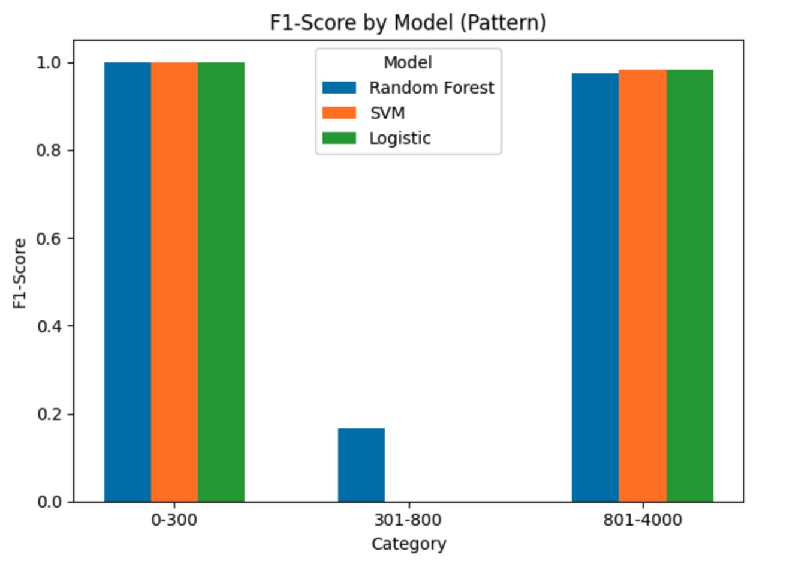
\includegraphics[width=0.75\linewidth]{Pattern Scenario ML Model F1_Score.png}
    \caption{Pattern Scenario ML Model F1 Score}
    \label{fig:enter-label}
\end{figure}



\section{Performance Evaluation}
%      \item What experiments are you going to run?
   %   \item What criteria and metrics are you going to use to evaluate your solutions?
\subsection{Simulation Setup}
\paragraph{}
In both the random and pattern behavior scenarios, the network simulation is configured with consistent parameters to ensure comparability of results. The node configuration comprises one WiFi access point node and a variable number of WiFi station nodes—specifically, setups with two and four nodes to represent different devices within the network. For channel and physical layer (PHY) settings, the ConstantSeedPropagationDelayModel is utilized to simulate propagation delay, while the FriisPropagationLossModel is adopted to account for signal attenuation over distance. Mobility within the network is defined by a stationary grid setup, with nodes positioned at the origin (0.0, 0.0) and spaced 5.0 meters apart, signifying a static environment where the devices do not change location. IP addressing follows a standardized schema with the base address set to 192.168.239.0 and a subnet mask of 255.255.255.0, which is typical for local area networks. Lastly, each simulation runs for a duration of 900 seconds, equivalent to 15 minutes, providing a sufficient time frame to observe and analyze the network behavior under both scenarios.

\paragraph{}
In the Pattern Scenario, WiFi is set to the 802.11b standard, with bandwidth allocation of 1 Mbps increasing to 5.5 Mbps when allocated. The traffic is structured, with an iPad and Smart TV each assigned specific IPs and sending UDP packets at regular 1-second intervals, but with different packet sizes of 1024 and 2048 bytes respectively. In contrast, the Random Scenario uses the same WiFi standard but differs by assigning random data rates ranging from 1 to 11 Mbps. Here, the iPad and Smart TV send packets at a much faster rate of 0.1 seconds, while additional devices like a laptop and cell phone send packets at 5 and 1-second intervals with smaller packet sizes of 512 and 256 bytes, respectively. This reflects a more chaotic network load, typical of actual home environments where device usage and internet demands fluctuate unpredictably.

\subsection{Result Analysis}

\begin{figure}[H]
    \centering
    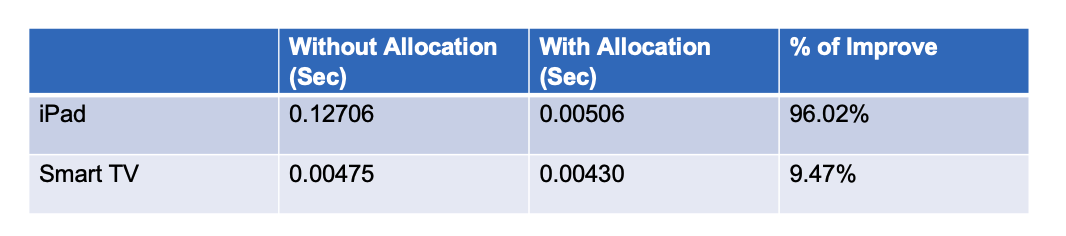
\includegraphics[width=0.75\linewidth]{Latency Result.png}
    \caption{Simulation Latency Result}
    \label{fig:enter-label}
\end{figure}

\begin{figure}[H]
    \centering
    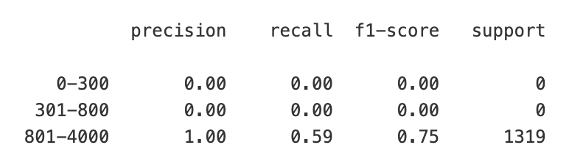
\includegraphics[width=0.6\linewidth]{Pattern Prediction.png}
    \caption{Bandwidth Prediction on Pattern Scenario
}
    \label{fig:enter-label}
\end{figure}

\paragraph{}
Post-simulation, pcap network traffic files from NS3 are analyzed, and the initial latency—rather than average latency—for each device is calculated. The results (Figure 7) show that pre-allocating bandwidth significantly improves device performance. For the iPad, without bandwidth allocation, the latency is recorded at 0.12706 seconds. With bandwidth allocation, this latency dramatically drops to 0.00506 seconds, resulting in a 96.02\% improvement. This suggests that bandwidth allocation can substantially enhance the network performance experienced by the iPad. In the case of the Smart TV, the improvement is more modest. The latency without allocation stands at 0.00475 seconds, improving to 0.00430 seconds with allocation, which constitutes a 9.47\% improvement. Although the percentage improvement for the Smart TV is less compared to the iPad, it still indicates a positive impact of bandwidth allocation.


\paragraph{}
The NS3 simulation for the random behavior scenario failed to generate correct outputs, which has impeded a direct evaluation of the machine learning model's performance in such conditions. Nevertheless, preliminary analysis indicates that the machine learning model's efficacy in random scenarios would likely be suboptimal. This inference stems from the inherent complexity of random behavior, which does not lend itself well to pattern recognition and prediction — the strengths of the current model. In the pattern scenario, despite the model's excellent precision, as reflected in the classification report (Figure 8), with a precision of 1.00, the recall is 0.59. This reveals the model's limitation in identifying all true instances, with a consequent F1-score of 0.75 and support of 1319. This indicates that the model is proficient in its predictive accuracy for occurrences it has identified but could be improved in its comprehensive detection capabilities. It is postulated that inputting simulation results from a four-device scenario into the model could enhance its predictive performance, as evidenced by a potentially improved F1-score. Given the model's design for structured environments, the unavailability of accurate simulation results for the random scenario is not deemed significantly detrimental. The model's limited applicability in random settings suggests that focusing on structured, predictable network scenarios would be more beneficial, aligning with the system's intended use for smart bandwidth allocation.
    
\section{Conclusion (Dec 8, 2023)} %(with dates)
\subsection{Solution's Conclusion}
\paragraph{}
The machine learning (ML) prediction results indicate a notably promising outcome when applied to a pattern usage scenario. This suggests that when device usage and network traffic follow a predictable pattern, ML algorithms can effectively anticipate bandwidth requirements and contribute to significant improvements in network performance. Specifically, the ML model can accurately predict network load, allowing for preemptive bandwidth allocation and resulting in enhanced network efficiency. On the other hand, in random usage scenarios, where device activity and network demands are unpredictable, the ML predictions appear to have little to no beneficial impact. The unpredictable nature of traffic in such scenarios makes it challenging for the ML model to make accurate predictions, which in turn limits the potential for performance improvements.
\paragraph{}
The experiment's results showcase a dramatic 96\% reduction in latency for the initiation of network connections on the iPad with bandwidth allocation, highlighting the effectiveness of the proposed solution in managing network resources more efficiently. The Smart TV also benefits from the bandwidth allocation, albeit to a lesser extent, with a 9.5\% latency reduction upon connection initiation.
\paragraph{}
These findings underscore that a home network characterized by patterned behavior can significantly benefit from the proposed ML-based solution, as it can leverage predictable usage patterns to optimize bandwidth distribution. Conversely, a home network with random device behavior might not see the same level of efficiency gains, as the ML model's ability to improve network performance is constrained by the lack of predictable patterns.
\paragraph{}
Overall, the results confirm that the network's efficiency can be greatly enhanced in specific scenarios by employing a targeted ML approach for bandwidth management. This underscores the importance of understanding network traffic patterns to effectively apply ML solutions for network performance optimization.

\subsection{Future Work}
\paragraph{}
The future work for this Smart Bandwidth Allocation project is set to focus on three pivotal enhancements to elevate network management into a new era of automation and intelligence. 
\paragraph{}
First, the project aims to develop a system that will enable the machine learning models to update automatically as they ingest new data regularly. This will ensure that the models continuously evolve and adapt to changing usage patterns, maintaining their accuracy and relevance. Second, there will be a concerted effort to integrate the machine learning predictive analytics directly into network management software. This will allow for dynamic bandwidth allocation based on real-time data and forecasts, ensuring optimal network efficiency and user experience. Finally, the project seeks to deploy this advanced network management solution onto WiFi routers themselves. By embedding the software directly into the routers, the network hardware will become intelligent, capable of proactive self-management. This will reduce latency and improve overall network performance without the need for external control systems. 
\paragraph{}
These future developments are designed to realize the full potential of a smart bandwidth allocation system, creating a network that not only connects devices but also intelligently orchestrates their interaction to maximize efficiency and performance.

\newpage
\bibliographystyle{plain}
\bibliography{yourref}


\end{document}
